\documentclass[12pt]{article}
\usepackage[paperwidth=8.5in,paperheight=11in,margin=1in]{geometry}
\usepackage{float}
\usepackage{lipsum}
\usepackage{parskip}
\usepackage{bbding}
\usepackage{amssymb}
\usepackage{titlesec} 
\usepackage{graphicx}
\usepackage{hyperref}
\usepackage{setspace}
\usepackage[normalem]{ulem}
\usepackage[section]{placeins}
\usepackage[toc,page]{appendix}
\newcounter{subsubsubsection}[subsubsection]
\newcommand{\tline}{\hspace{-2.3pt}$\bullet$ \hspace{5pt}}
\hypersetup{colorlinks=true, linkcolor=black, urlcolor=blue}
\setlength{\parindent}{15pt} % Indent paragraphs (automatically)
\usepackage{pdfpages, caption}


\makeatother
\makeatletter
\setlength{\@fptop}{0pt}

\newcommand\tab[1][1cm]{\hspace*{#1}}

\definecolor{myRed}{RGB}{248, 0, 0}
\definecolor{myGreen}{RGB}{0, 208, 0} %full green too light -P
\definecolor{myBlue}{RGB}{0, 0, 248}

\begin{document}
	\begin{titlepage}
		\centering	
%		\vspace{.25cm}
    
    \begin{figure}[h]
      \centering
      
\includegraphics[width=0.38\linewidth]{assets/New_Logov1.png}
    \end{figure} 
  
  {\huge\bfseries The Coeur d'Alene Catfish: \\ Research Portfolio\par}
    
    \title{}
    \date{\vspace{-5ex}} %blank date -P
    \author{%
    	\makebox[.3\linewidth]{\Large\itshape Adrian Beehner}\\Team Manager\\
    	\and \makebox[.3\linewidth]{\Large\itshape Samantha Freitas}\\Designer\\
    }
    \let\newpage\relax\maketitle %don't make a new page -P
    \maketitle		
    
    \vspace{1cm} 
    
    {\scshape\Large 
      May 2018 - August 2018 \\
      Autonomous Robotic Submarine Project\\ 
      Sponsors - Idaho Water Resources Research Institute, United States Geologic Survey, UofI \\
      Supervisor - Dr. John Shovic
      \par}
    
     \vspace{1cm} 
    
    \begin{figure}[h]
      \centering
      
\includegraphics[width=0.6\linewidth]{assets/uislogan.png}
    \end{figure} 
  
		\vfill		
	\end{titlepage}

	\tableofcontents
	\newpage
	
	\section{Introduction}
	
		\subsection{Goal}
		Autonomous navigation and sampling of lake sediment in North Idaho lakes up to 1200 feet in depth. Project is being operated in cooperation with Gizmo and CDA Maker Space
	
		\subsection{Project Summary}
		The western region of the United States has been home to expensive mining operations, and there is an abundance of abandoned hard rock mines that fill this landscape. These mines contain dangerous toxins that contaminate nearby soils and water. Thus a large portion of headwater streams in the Western United States have been effected by this. These toxins and metals can be transmitted to lake basins, which can become repositories for a large quantity of sediment associated metals. Coeur d'Alene lake in Northern Idaho, where silver and lead mining in the South fork of Coeur d'Alene River has carried heavy metal contaminated sediments to the lakebed. Thus in Coeur d'Alene lake this is a prominent issue, and while these issues are apparent there, it is not just this lake that has this problem. Legacy Contamination within river beads is a problem on an international scale. Computer models also do not provide an accurate characterization of the transport of contamination, a more direct sensing of contamination is required. This is where the research for this project comes into play, to develop the Coeur d'Alene Catfish, which is an autonomous robotic drone that is capable of reading water quality information from Coeur d'Alene lake, and other deep water lakes. The end result then should be the development (key word is development, not completion) of a submarine that can provide autonomous deployment within Coeur d'Alene lake and other deep water lakes. Reservoirs are also desired as well, which can be fairly difficult to navigate due to the problematic kinetic nature of the environment. This in turn allows public to the supervision of water bodies in local communities as well. The results from such surveys conducted by the drone will be shared with other interested stakeholders, this will include the Idaho Water Department of Environmental Quality (IDEQ) and Coeur d'Alene Tribe.\\
		The research focuses on creating and/or starting beginning development into the infrastructure of an autonomous submarine (and sensor technologies). Thus the long term goal is a fully functional autonomous submarine that can collect water quality data in deep-water lakes and reservoirs. The short term goal is to develop the "CDA Catfish", submarine that can perform underwater surveys by continuously sampling a variety of water quality variables (oxygen, pH, temperature, etc).\\
		Interested parties/sponsors for pursuing this research include the Idaho Water Resource Research Institute, the United States Geologic Survey, and the University of Idaho. The research is also in cooperation with Gizmo, Coeur d'Alene Maker Space.\\
		Documentation and code for the project can be found at \url{https://github.com/TimetoPretend54/The-Coeur-d-Alene-Catfish}
		
		\subsection{Document Purpose}
			This document is a research portfolio for the University of Idaho Research Project for the Computer Science Department pertaining to underwater autonomous navigation. The purpose of this documents is to outline the methodology, design, decisions, evaluations, and to keep a record of this project. It defines the terms used, outlines the scope of the project, details of specific design choices, meeting minutes, project learning, design goals, specification and constraints, system diagrams, analysis of alternatives, engineering modeling, manufacturing/assembly plan, experimental design, data analysis, balance sheet, and other items.
		
		\subsection{Definition of Terms}
			\begin{itemize}
				\item \textbf{G2X} - A remotely operated underwater vehicle developed by Gizmo-cda, a makerspace located in Coeur d'Alene Idaho. The vehicle itself operates with 5 thrusters, with a Raspberry Pi (Model 3) as the SBC (Single Board Controller), alongside additional components. Components are located within the navigation module of the G2X. The vehicle can be operated via a controller (using the Pygame Python library and a Playstation 4 Controller), requiring a tether (handling gear) to provide the input, or can be run autonomously with a program, running on the G2X's Raspberry P (no tether), or a host computer (tether required). Operational Time is 6 hours on full charge, thrusters and raspberry pi operate on separate batteries, 8 hours for Pi, 6 hours for thrusters.Software for operating the software is provided courtesy of Gizmo, located at \url{https://github.com/gizmo-cda/g2x-submarine-v2}
				\item \textbf{Navigation Module} - Module located within the G2X that houses the the primary components of the vehicle, components are a Raspberry Pi 3, PiSenseHat (sensor module that includes internal pressure, temperature, compass, accelerometer, and gyroscope readings), a PWM Hat (for handling the PWM thrusters), an Arduino Nano for reading voltage, 5 Electronic Speed Controllers (ESC), a power regulator, pressure, temperature sensor for external treadings, and a Pi Camera V2 NoIR (video streaming).
				\item \textbf{ROS} - Robot Operating System. It is a robotics middle collection of software frameworks for robot software development. ROS Node is just an executable file within a ROS package, utilizing the ROS client library to communicate with other nodes\\ (https://en.wikipedia.org/wiki/Robot\textunderscore Operating\textunderscore System)
				\item \textbf{Raspberry Pi} - Single Board Computer (SBC) that is a small, compact (about the size of credit card), and affordable computer that promotes a wide variety of applications. The Operating System (OS) that runs on the Pi is Raspberian, which is based on the Debian operating system (Linux Distribution).\\ (https://en.wikipedia.org/wiki/Raspberry\textunderscore Pi)	
				\item \textbf{Arduino} - Open source computer hardware and software company, project, and user community that designs and manufactures 		single-board microcontrollers and microcontroller kits for building digital devices and interactive objects that can sense and control objects in the physical world\\ (https://en.wikipedia.org/wiki/Arduino)		
				\item \textbf{Handling Gear} - Gear and metal frame for lowering the G2X into the water (via a wench), a fiber optic tether that provides video streaming, alongside controller output (Playstation 4 Controller). The gear provides simple switches for retracting and extracting both the wench and tether. Powered by a 12V car battery, and operational for more than 36+ hours. The handling gear has the communications module attached.
				\item \textbf{Communications Module} - A module that houses an additional raspberry pi, the module is a network interface for transferring data between the G2X and a host computer. It contains the Pi, external pressure/temperature sensor, 1 GB fiber optic media converter, 4-port GB switch, Wide-angle camera, real time clock, power supply (12V from handling gear).
				\item \textbf{TurtleBot} - TurtleBot is a low-cost, personal robot kit with open-source software. With TurtleBot, you’ll can build a robot that can drive around, see in 3D, and create applications.The TurtleBot kit consists of a mobile base, 2D/3D distance sensor, laptop computer or SBC(Raspberry Pi), and the TurtleBot mounting hardware kit.\\
				(https://wiki.ros.org/Robots/TurtleBot)
				\item \textbf{Octomap} - An efficient probabilistic 3D mapping framework based on octrees. It is a ROS Library that implements a 3D occupancy grid mapping approach providing data structures and mapping algorithms in C++. The map implementation is based on an octree (tree data structure in which each internal node has exactly eight children). \\
				(https://wiki.ros.org/octomap)
				\item \textbf{Moveit!} - A motion planning framework.It is a software framework for mobile manipulation, including utilizing advances in motion planning, manipulation, 3D perception, kinematics, control and navigation. Thus providing a simple platform for developing robotics applications.\\
				(https://moveit.ros.org/)
				\item \textbf{SLAM} - Simultaneous localization and mapping. SLAM is a computational problem of constructing or updating a map of an unknown environment while simultaneously keeping track of an agent's location within it. There are several algorithms known for solving it (at least approximately).\\
				(https://en.wikipedia.org/wiki/Simultaneous\textunderscore localization\textunderscore and\textunderscore mapping)
			\end{itemize}
		
		\subsubsection{ROS - Additional Info}
		The Robot Operating System contains many essential features, including: hardware abstraction, low-level device control, message-passing between processes, and package management. ROS nodes are written in either C++ or Python. ROS is primarily supported on Ubuntu Linux, with other major OS being designated as "Experimental". The underwater research project will be using ROS Kinetic Kame (2016) as its ROS version, due to its supported features and stability. 
		
		\newpage
	
	\section{Meetings and Minutes}
	Weekly action items and summaries of progress made are detailed below. Furthermore, subsections discuss what was helpful and what was not during these meetings. Discussion of attendance and participation, as well as contribution and discussion topics are discussed below.
	
		\subsection{5/15/2018 Team Meeting 1 Notes}
		
			\noindent
			Adrian and Samantha present at 9:00 am, Dr. Shovic joined at 9:03 am. Meeting was held at the Innovation Den in Coeur d'Alene, everyone was accounted for and prepared. Purpose of the meeting was to discuss beginning of the research project, to outline goals, expectations, and any other additional information required to start the research project.
		
			\noindent
			Project Scope Breakdown (Dr. Shovic, Adrian, Samantha started 9:05 am):
			
			\noindent
			\begin{itemize}
				\item Submarine Delivery 
				\begin{itemize}
					\item Submarine in Gizmo office
					\item Will be delivered tomorrow
					\begin{itemize}
						\item Keep submarine in lab
					\end{itemize}
				\end{itemize}
				\item Notebook
				\begin{itemize}
					\item Samantha and Adrian need one
				\end{itemize}
				\item Research
				\begin{itemize}
					\item Need to write a research paper
					\item At end of summer
					\item All teammates
				\end{itemize}
				\item Logbook
				\begin{itemize}
					\item Need to write about everything done to submarine
					\item Clearly designed and obvious
				\end{itemize}
				\item Three Main Items to Research
				\begin{enumerate}
					\item Do Field Trials
					\begin{itemize}
						\item June = testrun of Gizmo Submarine
						\item July = team software running on it
					\end{itemize}
					\item Get Team's Software Running on Submarine
					\item Fully Document Submarine
					\begin{itemize}
						\item Research Paper
					\end{itemize}
				\end{enumerate}
				\item Goals
				\begin{itemize}
					\item Adrian - head of project
					\begin{itemize}
						\item Allocate resources to make goals
					\end{itemize}
					\item Get current toolchain working (Gizmo)
				\end{itemize}
				\item Documentation
				\begin{itemize}
					\item Essential for project
					\item Set up our own Google Drive for University of Idaho Catfish
					\item Blank documents for what we know we need
					\item GitHub Repo
					\item Research portfolio
					\item Operations manual
					\item Need good documentation as Submarine may be senior project for next academic year
					\item Document Sub-systems of submarine
				\end{itemize}
				\item Cooperate
				\begin{itemize}
					\item University of South Dakota has expressed interest in similar research
				\end{itemize}
				\item Events
				\begin{itemize}
					\item Bayview visit, Dr. Shovic will be visiting next week on Monday
					\item 26th of July
					\begin{itemize}
						\item Vice President of Research
						\begin{itemize}
							\item Presentation for her
						\end{itemize}
						\item Schedule when Field Tests Occur
						\begin{itemize}
							\item July 24th = Trials
						\end{itemize}
					\end{itemize}
				\end{itemize}
				\item Architecture
				\begin{itemize}
					\item Graphic with items labled on it
					\item Two types:
					\begin{enumerate}
						\item With downward camera
						\item Without downward camera
					\end{enumerate}
				\end{itemize}
				\item Trials
				\begin{enumerate}
					\item June-Week of the 25th
					\begin{itemize}
						\item Provide more for operations manual and get experience
					\end{itemize}
					\item July - Late July (25th)
					\begin{itemize}
						\item Alternative Date: August 8th
						\item Also still tethered
					\end{itemize}
					\item So what for 2nd Field Test?
					\begin{itemize}
						\item Some amount of autonomous navigation
						\item No GPS system at that point
					\end{itemize}
				\end{enumerate}
				\item Submarine
				\begin{itemize}
					\item Sensors, communicator, actuator
					\item Sensor
					\begin{itemize}
						\item Camera in front
						\begin{itemize}
							\item Edited a lot, multiple resolutions
							\item Have 2TB disk on hand
						\end{itemize}
						\item Compass/Accelerometer
						\begin{itemize}
							\item Next to useless
							\item Due to metal casing
						\end{itemize}
						\item Sonar
						\begin{itemize}
							\item Need to look at research papers
							\item Four sonars? (up, down, left, right)
							\item Up = GPS station keep (water drone with GPS receiver)
							\item Listen to sonar and center itself
						\end{itemize}
						\item Acoustic Modem (ACM)
						\begin{itemize}
							\item Status data up
							\item GPS data down
							\item 30 k/bits a second or 90 k/bits
							\item Might be able to use as navigational thing
						\end{itemize}
						\item Before 2nd Trial
						\begin{itemize}
							\item 100 ft range with these sonars - Can we test?
							\item Large water through?
							\item Not large enough or submarine likely
							\item But can test sonars at least
						\end{itemize}
					\end{itemize}
					\item Document all the wires
				\end{itemize}
				\item Pod
				\begin{itemize}
					\item Built by folks in Boise
					\item Wireless interference from pod to submarine is a concern
					\item Create software to communicate data (bi-directional link)
					\item Arduino for Pod
					\begin{itemize}
						\item Thus don't need ROS for Arduino
					\end{itemize}
					\begin{itemize}
						\item TCP/IP packet data sending
						\item 1,024 bytes of data packages
					\end{itemize}
					\item RPI (Raspberry Pi 3)
					\begin{itemize}
						\item Wifi
						\begin{itemize}
							\item 2.4 GHz
							\item highest water absorption frequency
							\item Tens of centimeters
						\end{itemize}
						\item Wifi Arduino Shield on Arduino (Pod)
						\begin{itemize}
							\item Where data comes from
						\end{itemize}
					\end{itemize}
					\item Metal Issue
					\begin{itemize}
						\item Nothing can transmit in/out usually
						\item Piece of metal between submarine and pod
						\begin{itemize}
							\item Maybe cut out circular hole in metal probably?
						\end{itemize}
					\end{itemize}
					\item Accuracy for sensors in Pod
					\begin{itemize}
						\item 10 Bits
					\end{itemize}
					\item Prototype GPS data to submarine through laptop
				\end{itemize}
				\item Effort
				\begin{itemize}
					\item Take a look at: Drone Controller Cards
					\begin{itemize}
						\item Card that stabilizes drone
						\item Corrects yaw, roll, pitch
						\item Keep submarine flat 
						\item Submarine will act like a flying drone (just underwater)
						\item Interfaced with ROS
					\end{itemize}
					\item Will have accelerometer
					\item Simplify control system
				\end{itemize}
				\item Research Questions
				\begin{itemize}
					\item How the heck can we build a navigation system (with a cheap sonar)?
					\item Debugging?
					\item Implementing full tool-chain
					\begin{itemize}
						\item Turn into ROS interface
					\end{itemize}
				\end{itemize}
				\item Boise - Conference Call
				\begin{itemize}
					\item Next Wednesday May 23rd
				\end{itemize}
				\item Other Questions
				\begin{itemize}
					\item What type of computer?
					\begin{itemize}
						\item Which OS, specifications, required software, etc?
					\end{itemize}
				\end{itemize}
				\begin{figure}[!htb]
					\centering
					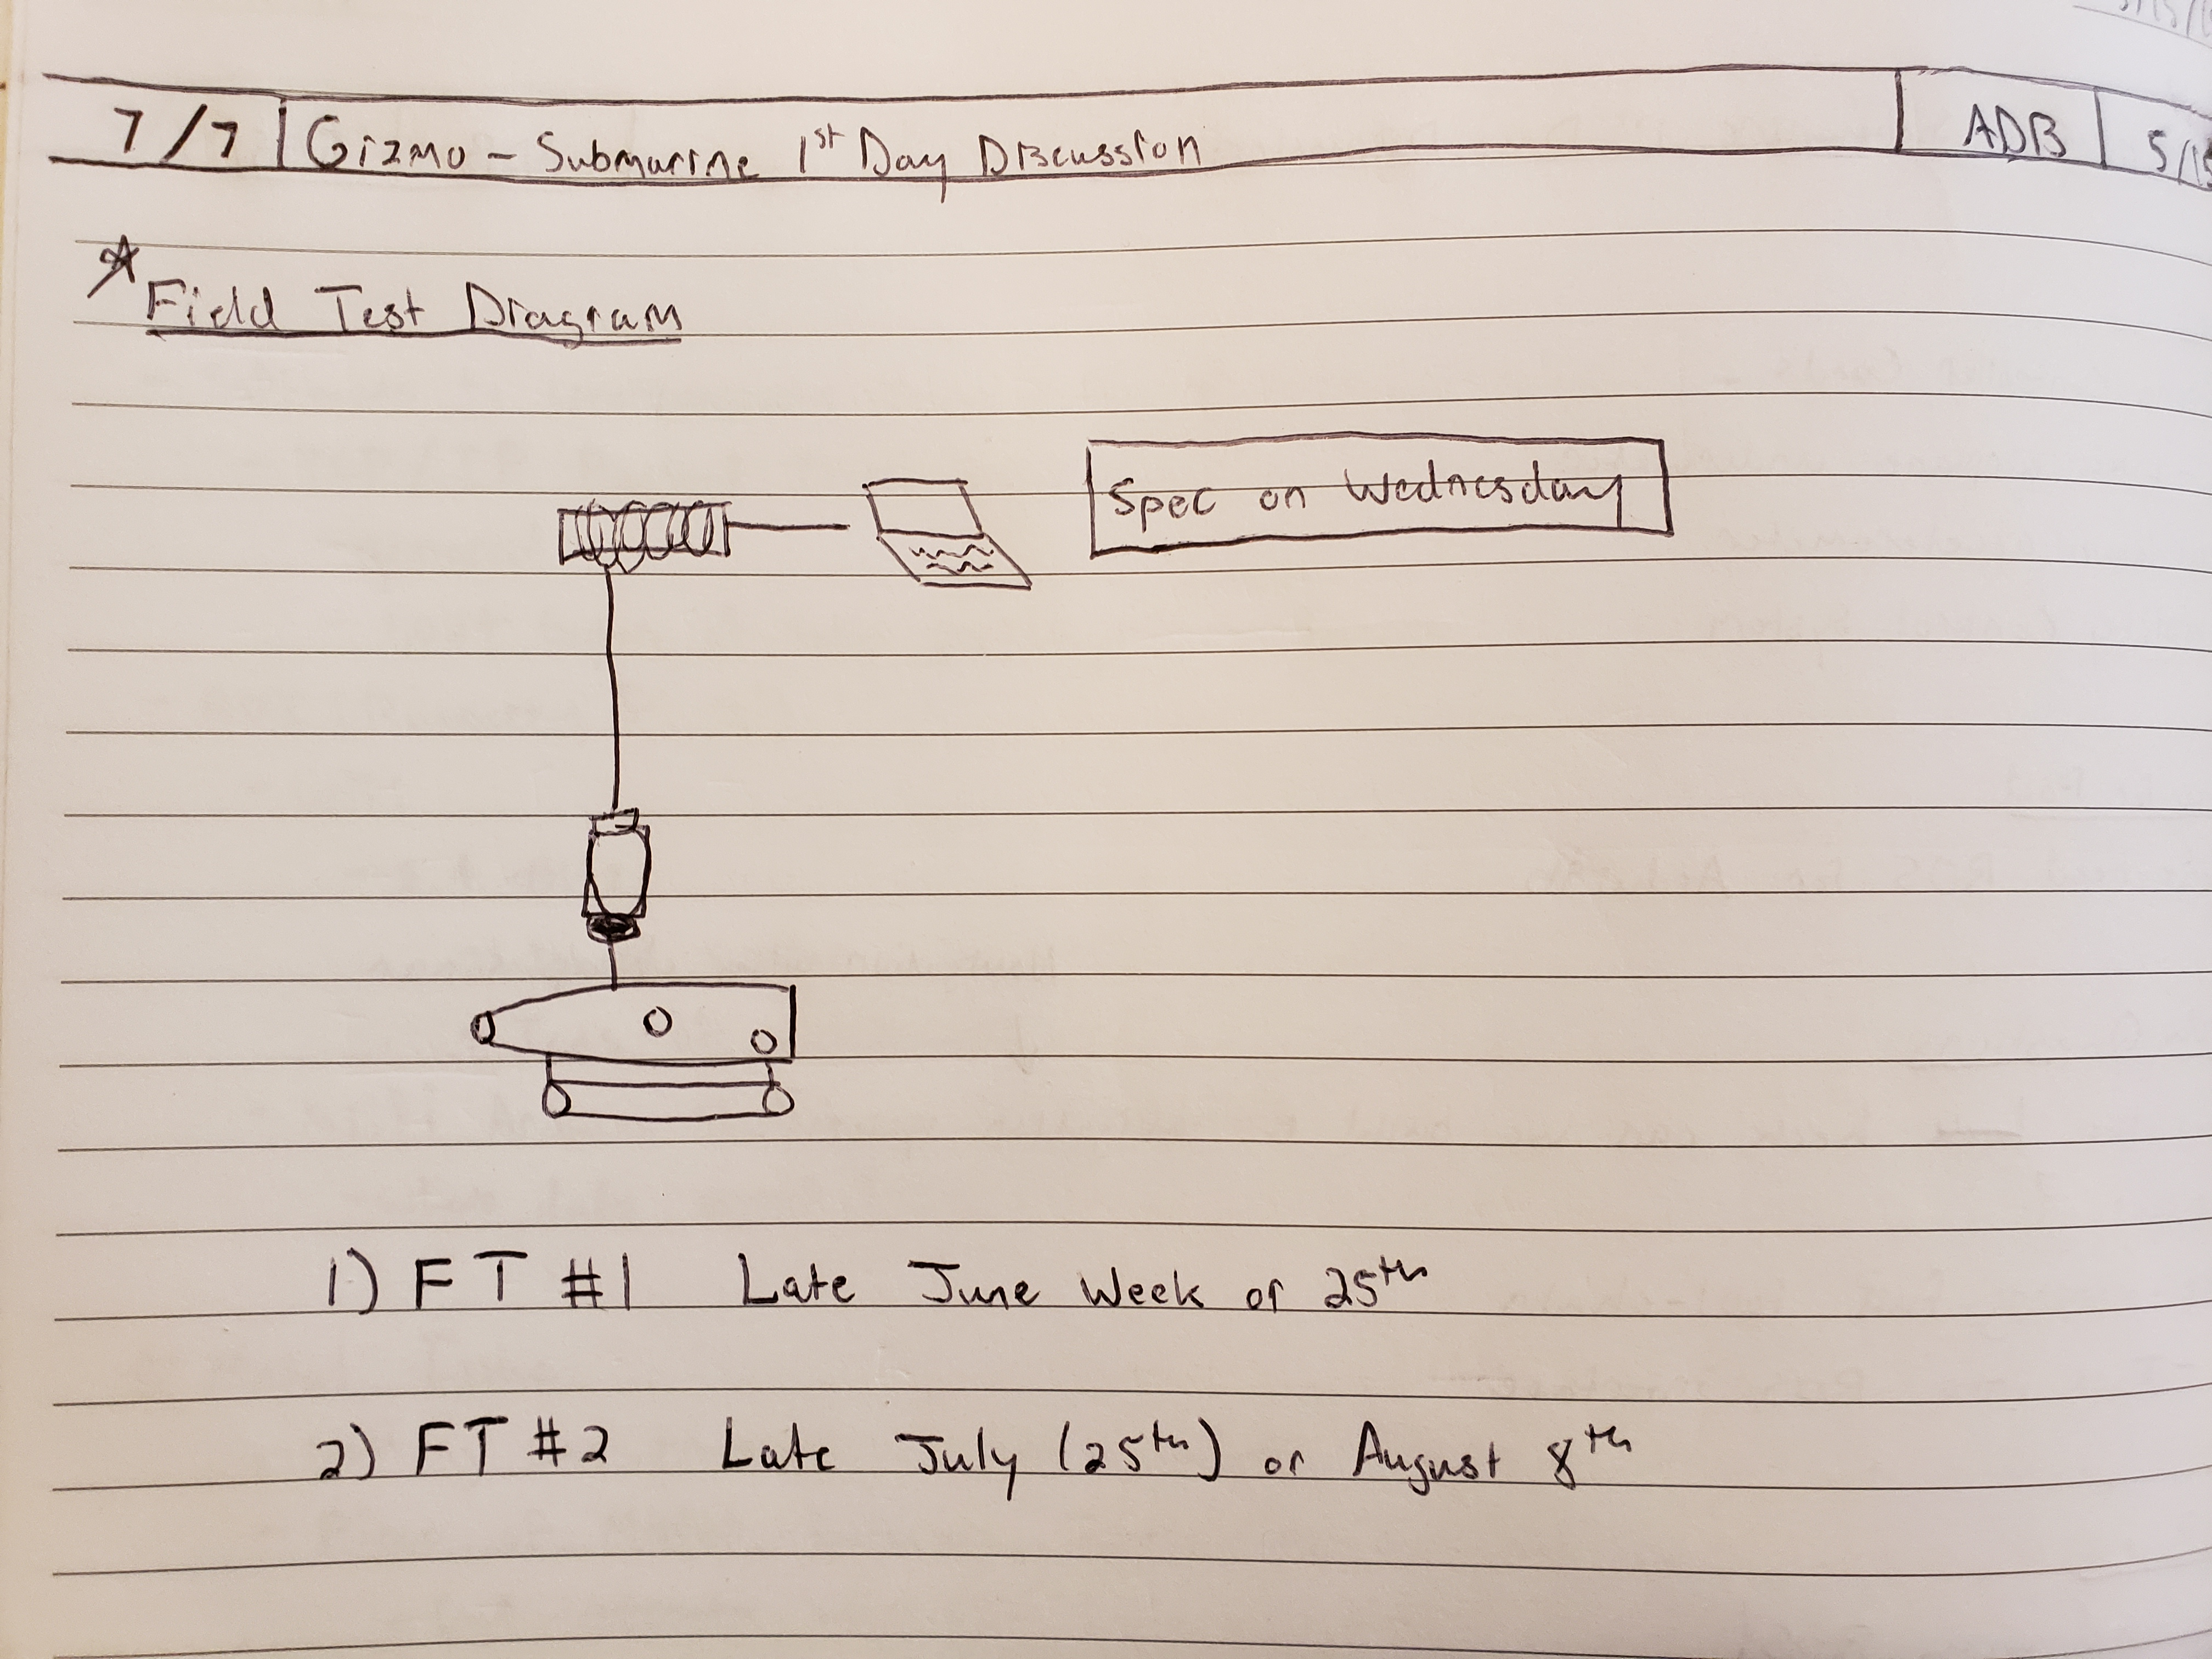
\includegraphics[width=130mm]{assets/Field_Test_Diagram.jpg}
					\caption{5/14 Field Test Diagram \label{overflow}}
				\end{figure}
			\end{itemize}
		
			\noindent
			\\Meeting concluded at 11:00 am
			
			\clearpage
			
		\subsection{5/24/2018 Team Meeting 2 Notes}
		
			\noindent
			Adrian and Samantha present at 9:30 am, the meeting was held in the classroom at the Innovation Den, Dr. Shovic arrived at 9:29 am. Meeting attire was required to be professional/formal, thus both teammates wore appropriate attire. Meeting agenda were printed out beforehand to keep meeting organized and structured.
			
			\noindent
			The purpose of the meeting was to discuss ideas about the project, such as the acoustic modem, GPS system, water tanks, laptop specs, Wi-Fi in water, sonar sensors, Gizmo assistance, and budget decisions.
			
			\noindent
			Meeting began at 9:31 am, everyone present, with printed meeting agendas for everyone:
			
			\noindent
			\begin{itemize}
				\item Requirements for Catfish Logo
				\begin{itemize}
					\item Clean and abstract
					\item University of Idaho "I" logo involved
					\item Needs to be easily recognizable to "know" submarine
					\item Mascot = catfish (maybe think like GitHub)
					\item Color and black and white versions
					\item Decal on side of submarine
				\end{itemize}
				\item Awareness of Project
				\begin{itemize}
					\item Scientific vs creative
					\item Depends on the environment
					\item Scientific community vs general public
				\end{itemize}
				\item Bayview - Submarine Tour
				\begin{itemize}
					\item Tours only for American citizens
					\item Huge submarines (20 ft long)
					\item Project with them?
					\begin{itemize}
						\item Maybe, they have fully autonomous submarine
						\item Navigation, buoys hung 3-4 miles under lake, it gets GPS signals from them and send the data to the submarine
						\item Trilateration to determine submarine location
						\item Use their system to navigate the Gizmo submarine
						\item Very difficult to get research money 
						\item Office of Naval Research
					\end{itemize}
				\end{itemize}
				\item DIY Boat
				\begin{itemize}
					\item Took boat of some kind
					\item Circular boat with four propellers
					\item Maybe just provide a design/feasibility of building one
					\item Propellers separated by 90 degrees
					\item Four motors allows to stay in one position
					\item Need to know feasibility but not practical/physical use (block diagrams)
				\end{itemize}
				\item Sonars
				\begin{itemize}
					\item Naval Base might be able to donate sonars
					\item Have currently 3 Maxbotix sonars, need 3 more
					\item So 6 total sonars (up, down, left, right, forward, backward)
					\item 3D print sensor holders
					\item Need to publish/subscribe all of them
				\end{itemize}
				\item Acoustic Modem
				\begin{itemize}
					\item Want it on the boat when launching submarine
					\begin{itemize}
						\item Wi-Fi connection on boat?
						\item 1-Mile connection
					\end{itemize}
					\item Simulate:
					\begin{itemize}
						\item Functions receives info
						\item Receives info from socket
					\end{itemize}
					\item Modular manner (one routine and swap it out)
					\item Idea:
					\begin{itemize}
						\item Analog to digital
						\item Transmit low data
						\item Sonar ultrasonic sensors
						\item Ultrasonic transducer?
					\end{itemize}
				\end{itemize}
				\item Water Tank
				\begin{itemize}
					\item Get water tank (small)
					\item What about docking?
					\item Will have to determine a location 
					\item Gizmo tank will be best!
				\end{itemize}
				\item June Trial
				\begin{itemize}
					\item Figure out where we want to take it
					\item So need Field Test 0!
					\item Launch before June 26th for testing
				\end{itemize}
				\item Laptop Specs
				\begin{itemize}
					\item Get laptop ordered ASAP
					\item Have Tim set it up (Ubuntu 16.04, ROS, Gazebo, Octomap)
				\end{itemize}
				\item Available Wires for Submarine
				\begin{itemize}
					\item Three to four needed for Acoustic Modem
					\item Two lines for sonar sensors
					\item Two antenna lines (sensor pod)
					\item One external Wi-Fi antenna
					\item Twenty three extra wires
				\end{itemize}
				\item Wi-Fi
				\begin{itemize}
					\item Arduino Wi-Fi shield good to go!
					\item Need peer-to-peer connection
					\item Need another Wi-Fi dongle with external atenna
				\end{itemize}
				\item Goals
				\begin{itemize}
					\item Capability, NOT complete product
					\item Demonstrate some Autonomous Navigation
					\item Expected results: capability and results! 
					\item Design and document: future
				\end{itemize}
			\end{itemize}
		
			\noindent
			\\Meeting concluded at 10:50 am
			
			\clearpage
		
		\subsection{5/31/2018 Team Meeting 3 Notes}
			
			\noindent
			Adrian and Samantha present at 9:27 am, the meeting was held in the classroom at the Innovation Den, Dr. Shovic arrived at 9:28 am. Meeting attire was required to be professional/formal, thus both teammates wore appropriate attire. Meeting agenda were printed out beforehand to keep meeting organized and structured. Had some printer errors for the agendas however, team had to reprint the agendas. 
			
			\noindent
			The purpose of the meeting was to discuss the operations manual, the media event, upgrading the raspberry pi, and discussing the sensor pod. Also during the meeting address the sonar ideas about the submarine. Adrian provided handouts/diagrams about the sonar ideas. During the meeting went onto discuss the ideas of sonar.
			
			\noindent
			Meeting began at 9:15 am, everyone present, with printed meeting agendas for everyone:
			
			\noindent
			\begin{itemize}
				\item Next Wednesday
				\begin{itemize}
					\item Status meeting next week
					\item Water through
				\end{itemize}
				\item Operations Manual
				\begin{itemize}
					\item Get done by next week --> assistance from Adrian on software
				\end{itemize}
				\item Media Event - Field Trial One
				\item Wi-Fi Side
				\begin{itemize}
					\item Sensor pod being developed
					\item PVC pipe
					\item Two plastic pipes (make Wi-Fi transmission better)
					\item Metal bottom of submarine (issue)
				\end{itemize}
				\item Raspberry Pi 3B+
				\begin{itemize}
					\item Currently have Raspberry Pi 3B,"+" version provides a slightly higher clock rate
					\item Also need to upgrade to Raspbian Stretch (currently sub is running Jessie)
					\item Duplicate current image of submarine SD card
				\end{itemize}
				\item Sensor Pod
				\begin{itemize}
					\item Arduino AtMega2560 (tons of I/O)
					\item 8K of RAM
				\end{itemize}
			\end{itemize}
		
			\noindent
			\\Meeting concluded at 10:20 am
			
			\clearpage
	
	
		\subsection{6/5/2018 Team Meeting 4 Notes}
	
			\noindent
			Adrian and Samantha present at 9:27 am, the meeting was held in the classroom at the Innovation Den, Dr. Shovic arrived at 9:28 am. Meeting attire was required to be professional/formal, thus both teammates wore appropriate attire. 
			
			\noindent
			The purpose of the meeting was to discuss the operations manual (software side), discuss some short-term goals, current GitHub, a voltage monitor, taking apart the submarine, discussing trials next week, communication Arduino and Raspberry Pi, and finally Wi-Fi testing.
			
			\noindent
			Meeting began at 9:30 am, everyone present, with printed meeting agendas for everyone:
			
			\noindent
			\begin{itemize}
				\item Operations Manual
				\begin{itemize}
					\item No legal stuff need to be included in it
				\end{itemize}
				\item To-Do
				\begin{itemize}
					\item Add battery voltage sensors
					\item Monitor voltages and current (low: 11V, high: 13V)
					\item INA 3221 Grove Board
					\begin{itemize}
						\item Monitor current and voltage
						\item Measuring voltage possible
						\item Current difficult to measure
					\end{itemize}
				\end{itemize}
				\item GitHub
				\begin{itemize}
					\item Clean up code and put additional items in
				\end{itemize}
				\item Next Week
				\begin{itemize}
					\item Take tube out (where all components are)
					\item Anything we do
					\item Labeled neatly and clearly
				\end{itemize}
				\item Software Operations Manual
				\begin{enumerate}
					\item Current Software
					\item Our Software (ROS) Version -> be well documented
				\end{enumerate}
				\item Next Week - Trials
				\begin{itemize}
					\item Next Friday Field Trail 0, June 15th
					\item Field Trial One (End of June)
				\end{itemize}
				\item Code
				\begin{itemize}
					\item Communications between Raspberry Pi and Arduino 
					\item TCP/IP packets
					\item Or perhaps MQTT packets
					\item Mosquito on Raspberry Pi (publish/subscribe system)
				\end{itemize}
				\item Field Trial One
				\begin{itemize}
					\item Arduino in battery and baggie
					\item Strap it on the bottom of submarine
				\end{itemize}
				\item Test Raspberry Pi Wi-Fi Range
				\item Ping Wi-Fi
				\item Need to carry submarine around!
				\item Will tell us how "leaky" the signal is
			\end{itemize}
		
			\noindent
			\\Meeting concluded at 10:15 am
		
			\clearpage
	
	
		\subsection{IWRRI Meeting - July 26th Launch Discussion}
		
			\noindent
			Meeting located at the Harbor Center, Adrian and Samantha arrive at 10:00 am, the meeting was originally held in room 242 at the Harbor Center. Other guests were Charles Buck, Alan Kolok, and a few other individuals. However, Alan did not arrive on time, and was supposedly going to be 20 minutes late. Thus, we first went out to the dock at the Harbor Center and examined the boat. Then after 20 minutes Alan arrived.
			
			\noindent
			The purpose of the meeting was to discuss the operations and schedule for the July 26th launch. In particular discuss guests, procedures, timing, location, and other details.
			
			\noindent
			 Once Alan arrived we all sat outside on a table and the official meeting began at 10:20 am:
			
			\noindent
			\begin{itemize}
				\item July 25th - Maybe Bring Submarine a Day Early
				\begin{itemize}
					\item Need to get properly prepped and prepared for the event on July 26th
				\end{itemize}
				\item July 26th
				\begin{itemize}
					\item 9:00 am to 11:00 the event will be held
					\item Larry, Bob, John, and Charles will be on the launch boat
					\item 9:00 - 9:15 am
					\begin{itemize}
						\item Boat ride to Cougar Bay
						\item Drone launch --> 1 main message
					\end{itemize}
					\item Media boat
					\item Charles Buck
					\item 8 Passengers 
					\item Phil, Photographer, Reporter, additional reporter
					\item John? (Don't know which boat he is on yet
				\end{itemize}
				\item Wear Lifevests
				\begin{itemize}
					\item Must wear them in pictures
				\end{itemize}
				\item No Water Monitoring!
				\begin{itemize}
					\item We will focus on the Catfish launch itself
					\item SO there is only one main focus!
				\end{itemize}
			\end{itemize}
			
			\noindent
			\\Meeting concluded at 10:55 am
			
			\clearpage
				
			
		\subsection{7/10/2018 Team Meeting 5 Notes}
			
			\noindent
			Adrian and Samantha present at 9:26 am, the meeting was held in the classroom at the Innovation Den, Dr. Shoivc arrived at 9:29 am. Meeting attire was required to be professional/formal, thus both teammates wore appropriate attire. Meeting agendas were printed out beforehand to keep the meeting organized and structured.
			
			\noindent
			The purpose of the meeting was to discuss the large list of prior achievements we accomplished, such as the software controlling checking, thruster overloading fix, operations manual completion, etc. Other included talking about the access point needed for Arduino, current for the Pi, a software timer for the Pi to Arduino, the boat launch, another dock launch, the July 26th launch, and moving forward with the project.
			
			\noindent
			Meeting began at 9:29 am, everyone present, with printed meeting agendas for everyone:
			
			\noindent
			\begin{itemize}
				\item Meeting Time?
				\begin{itemize}
					\item Ends at 11:00 am
					\item There is a long meeting to go through
				\end{itemize}
				\item Operations Manual
				\begin{itemize}
					\item Turn instructions into a series of checklists 
					\item Fix/edit some issues that have been fixed now in the software
				\end{itemize}
				\item Access Point
				\begin{itemize}
					\item Works on Jesse, but doesn't work on Stretch
					\item MQTT Message Transmission --> can't load Mosquito on the Access Point Raspberry Pi
					\item Access Point battery questions: 5V? Battery concerns? Wattage?
				\end{itemize}
				\item Reading Current from Pi
				\begin{itemize}
					\item Add that device later down the line
					\item Fall time-line
				\end{itemize}
				\item Pi to Arduino
				\begin{itemize}
					\item Software timer
					\begin{itemize}
						\item If Arduino gets no command
						\item Longer than full cycle reboot
					\end{itemize}
					\item Bandwidth? Will that pose any kind of issue?
				\end{itemize}
			\end{itemize}
		
			\noindent
			\\Meeting concluded at 10:40 am
			
			\clearpage
			
	\newpage

	\section{Project Learning}
	Technologies used to solve problems are described below. Further discussion of these technologies are left in each section's subsections.
	
		\subsection{Team Info}
		A discussion of the various pieces of info that relates to team information is provided below.
		
		% Remove Bullets from item list
		{\renewcommand\labelitemi{}
			% Begin list
			\begin{itemize}
				\item \textbf{Project Name}
				\begin{itemize}
					\item CDA Catfish
				\end{itemize}
				\item \textbf{Team Members}
				\begin{itemize}
					\item Adrian Beehner
					\item Samantha Freitas
				\end{itemize}
				\item \textbf{Sponsor}
				\begin{itemize}
					\item Dr. John Shovic
				\end{itemize}
			\end{itemize}
		
		\begin{figure}[!htb]
			\centering
			
\includegraphics[width=105mm]{assets/Team_Info.png}
			\caption{Team Info \label{overflow}}
		\end{figure}
		}	
		
		\clearpage
		
		
		\subsection{Proof of Design}
		A discussion of the various components is shown below, providing evidence of components working together:\\
		
		% Remove Bullets from item list
		{\renewcommand\labelitemi{}
			% Begin list
			\begin{itemize}
				\item \textbf{\textit{Navigation Module}}
					\begin{itemize}
						\item[] \textit{Hosed in G2X Shell, responsible for thruster control/navigation\\}
						\item[] \textbf{Raspberry Pi 3B with G2X V2 Software}
						\begin{itemize}
							\item Single-Board Computer (SBC) running a Linux-based OS (Raspbian)
							\item Raspbian runs the "g2x-submarine-v2" software upon boot
							\item Raspberry Pi interfaced with PWM/Servo Hat (thus software can control the thrusters with specific repetitive timing pulses)
						\end{itemize}
						\item[] \textbf{PWM/Servo Hat for Raspberry Pi}
						\begin{itemize}
							\item Adds the capability to control 16 Servos with perfect timing
							\item Up to 1.6 KHz with 12 bit precision, all completely free-running
						\end{itemize}
						\item[] \textbf{Electronic Speed Controller (x5)}
						\begin{itemize}
							\item Controls and regulates the speed of an electric motor. It may also provide reversing of the motor and dynamic braking
							\item Interfaced with PWM/Servo Hat
						\end{itemize}
						\item[] \textbf{Connectors}
						\begin{itemize}
							\item 8-Pin Power Connector (all pins used)
							\item 12-Pin Com Connector (for fiber optic connection between navigation module and communication module, pins 8-12 unused)
							\item 16-Pin Auxiliary Connector (pins 4-16 unused)
							\item 16-Pin Thruster Connector (pins 16 unused)
							\item Pressure Sensor
						\end{itemize}
						\item[] \textbf{Misc.}
						\begin{itemize}
							\item Realtime Clock (I2C)
							\item Arduino Nano (read voltage)
							\item Power regulator
							\item Pi Camera V2\\\\
						\end{itemize}
					\end{itemize}
				\item \textbf{\textit{Communications Module}}
				\begin{itemize}
					\item[] \textit{Hosed in External Metallic Cylinder (attaches to mast), allows communication to Pi on navigation module\\}
					\item[] \textbf{Raspberry Pi 3B}
					\begin{itemize}
						\item Single-Board Computer (SBC) running a Linux-based OS (Raspbian)
						\item Acts as a access point for communication between Host PC and Navigation Module Pi
					\end{itemize}
					\item[] \textbf{Pi Sense Hat}
					\begin{itemize}
						\item Add-on board for reading internal pressure, temperature, compass, accelerometer, and gyroscope
					\end{itemize}
					\item[] \textbf{1 Gb (Gigabit) Fiberoptic Media Converter}
					\begin{itemize}
						\item Converts UTP Gigabit Ethernet to Fiber Optic
						\item Fiber lengths up to 2Km
						\item Wavelength: 1310nm
					\end{itemize}
					\item[] \textbf{4-Port Gb Switch}
					\begin{itemize}
						\item Allows different devices on a network to communicate
						\item 4 auto-sensing Gigabit Ethernet ports
						\item Non-blocking switching architecture
					\end{itemize}
					\item[] \textbf{Fiberoptic Tether}
					\begin{itemize}
						\item Provides Fiberoptic connection (2000 ft. of tether) to the Communicator on the Handling Gear
						\item Communicator provides media converter between Fiberoptic and Ethernet (external PC Ethernet connection) 
					\end{itemize}
					\item[] \textbf{Navigation Fiberoptic Cable Plugin}
					\begin{itemize}
						\item Provides the Fiberoptic cable plugin (user plugs in cable) between the communications module and navigation module
					\end{itemize}
					\item[] \textbf{Misc.}
					\begin{itemize}
						\item Pi Camera V2
						\item Realtime Clock (I2C)
						\item Power Supply (5V from fiber optic connection)\\\\
					\end{itemize}
				\end{itemize}
				\item \textbf{\textit{G2X Vehicle/Shell}}
				\begin{itemize}	
					\item[] \textit{Houses the Navigation Module, Navigation Cable Box, 5 Thrusters, Power Switches (PWM and Pi), Buoyancy Foam, and a 12V battery\\}
					\item[] \textbf{T100 Thruster (x5)}
					\begin{itemize}
						\item Underwater thruster designed for marine robotics (created by Blue Robotics)
						\item Over 5 lbs of thrust
						\item Durable enough for great ocean depths
						\item Brushless electric motor (PWM servo signal)
					\end{itemize}
					\item[] \textbf{Lumen Subsea Light for ROV/AUV (x2)}
					\begin{itemize}
						\item A 1500 lumen subsea LED light with servo signal control, daisy-chain connection for multiple lights, and smart over-temp protection
						\item Made by Blue Robotics
						\item Fully dimmable control using a PWM servo signal
					\end{itemize}
					\item[] \textbf{Navigation Cable Box}
					\begin{itemize}
						\item Deals with wiring for 8-Pin Power Connector, 16-Pin Auxiliary Connector, and 16-Pin Thruster Connector
						\item Hoses wires which are not water-resistant but are interfaced with Navigation Module via being attached to 
						\item Includes wires for Pi power and Thruster (PWM) power which then interface into the 8-pin power connector
						\item Wiring interfacing the 5 T100 Thrusters into a singular waterproof wire that connects into the 16-Pin Thruster Connector
						\item Wiring interfacing with the 2 Lumen Subsea Lights into a singular waterproof wire that connects into the 16-Pin Auxiliary Connector
					\end{itemize}
					\item[] \textbf{3 12V Batteries}
					\begin{itemize}
						\item Underneath main plate of the G2X Vehicle
						\item 2 +12 VDC to thruster (PWM) power switch
						\item 1 +12 VDC to CPU (Pi) power switch
						\begin{itemize}
							\item Provides power to Raspberry Pi and PWM thrusters
						\end{itemize}
					\end{itemize}
					\item[] \textbf{Buoyancy Foam}
					\begin{itemize}
						\item Machinable, hydrostatic pressure-resistant foams that provide buoyancy underwater\\\\
					\end{itemize}
				\end{itemize}
				\item \textbf{\textit{G2X Handling Gear}}
				\begin{itemize}	
					\item[] \textit{Houses the Communication Module, Storage Box, 12V Battery, Communicator, Reel (w/ Fiberoptic Cable), Winch, and Handling Wiring Box\\}
					\item[] \textbf{Storage Box}
					\begin{itemize}
						\item Simple plastic box to house tools for launching and retrieving G2X vehicle, opening up components, etc.
					\end{itemize}
					\item[] \textbf{12V Battery}
					\begin{itemize}
						\item Provides power to the Handling Wiring Box and Communicator
					\end{itemize}
					\item[] \textbf{Communicator}
					\begin{itemize}
						\item Media converter from Ethernet to Fiberoptic Cable and vice versa
						\item Translates the connection from the external PC to the Pi in the Navigation Box
					\end{itemize}
					\item[] \textbf{Reel w/ Fiberoptic Cable}
					\begin{itemize}
						\item 2000 ft. of Fiberoptic Cable on Reel to provide a tether and fiberoptic media connection (via external PC) with G2X Vehicle
						\item Can be reeled in/out via the Handling Wiring Box
					\end{itemize}
					\item[] \textbf{Winch}
					\begin{itemize}
						\item ATV Winch used to lower the G2X vehicle into a body of water and retrieve it from the surface (from the body of water)
						\item Reeled in/out via the Handling Wiring Box
					\end{itemize}
					\item[] \textbf{Handling Wiring Box}
					\begin{itemize}
						\item Box that provides controls for reeling in/out both the Fiberoptic tether/cable and Winch
					\end{itemize}
				\end{itemize}
			\end{itemize}
		}
	
		\noindent \\\\Diagrams that correlate to the information that is provided above discussing the proof of design is shown below. Images are provided in the diagram to help provide a visual for certain aspects.

		\begin{figure}[!htb]
			\centering
			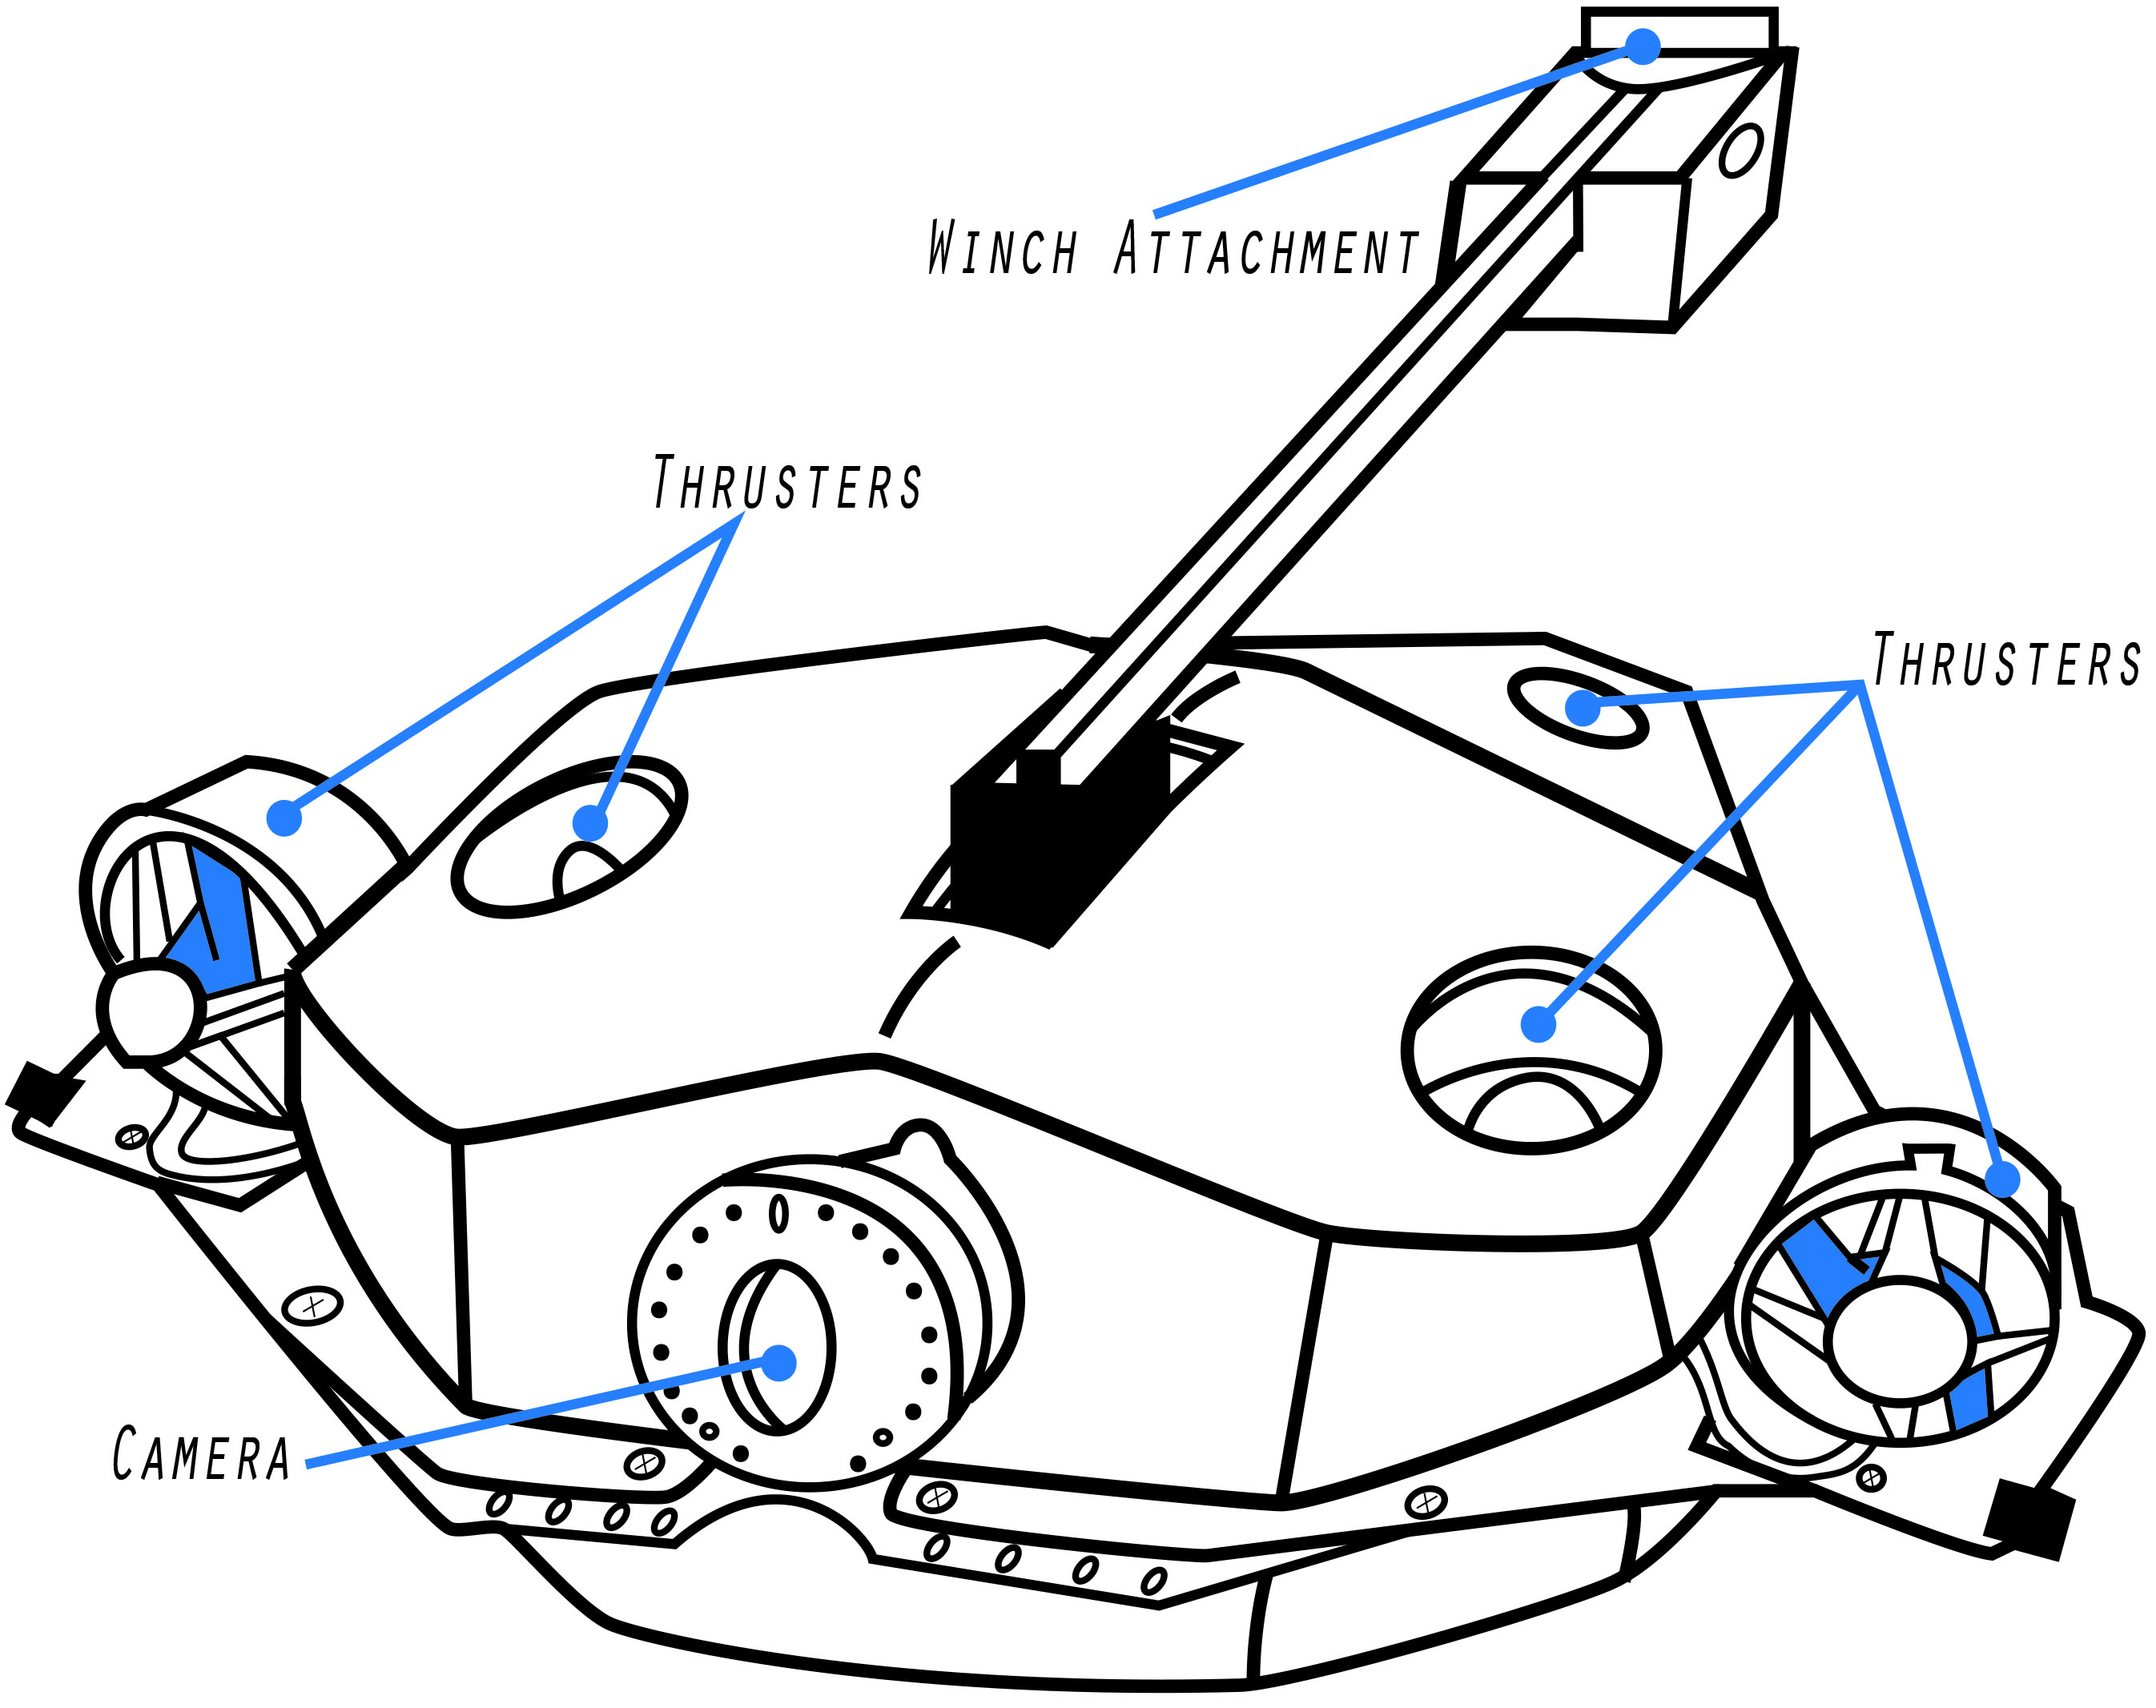
\includegraphics[width = 120mm]{assets/basic_sub.jpg}
			\caption{Proof of Design - G2X Vehicle Image 1 \label{overflow}}
		\end{figure}
	
		\begin{figure}[!htb]
			\centering
			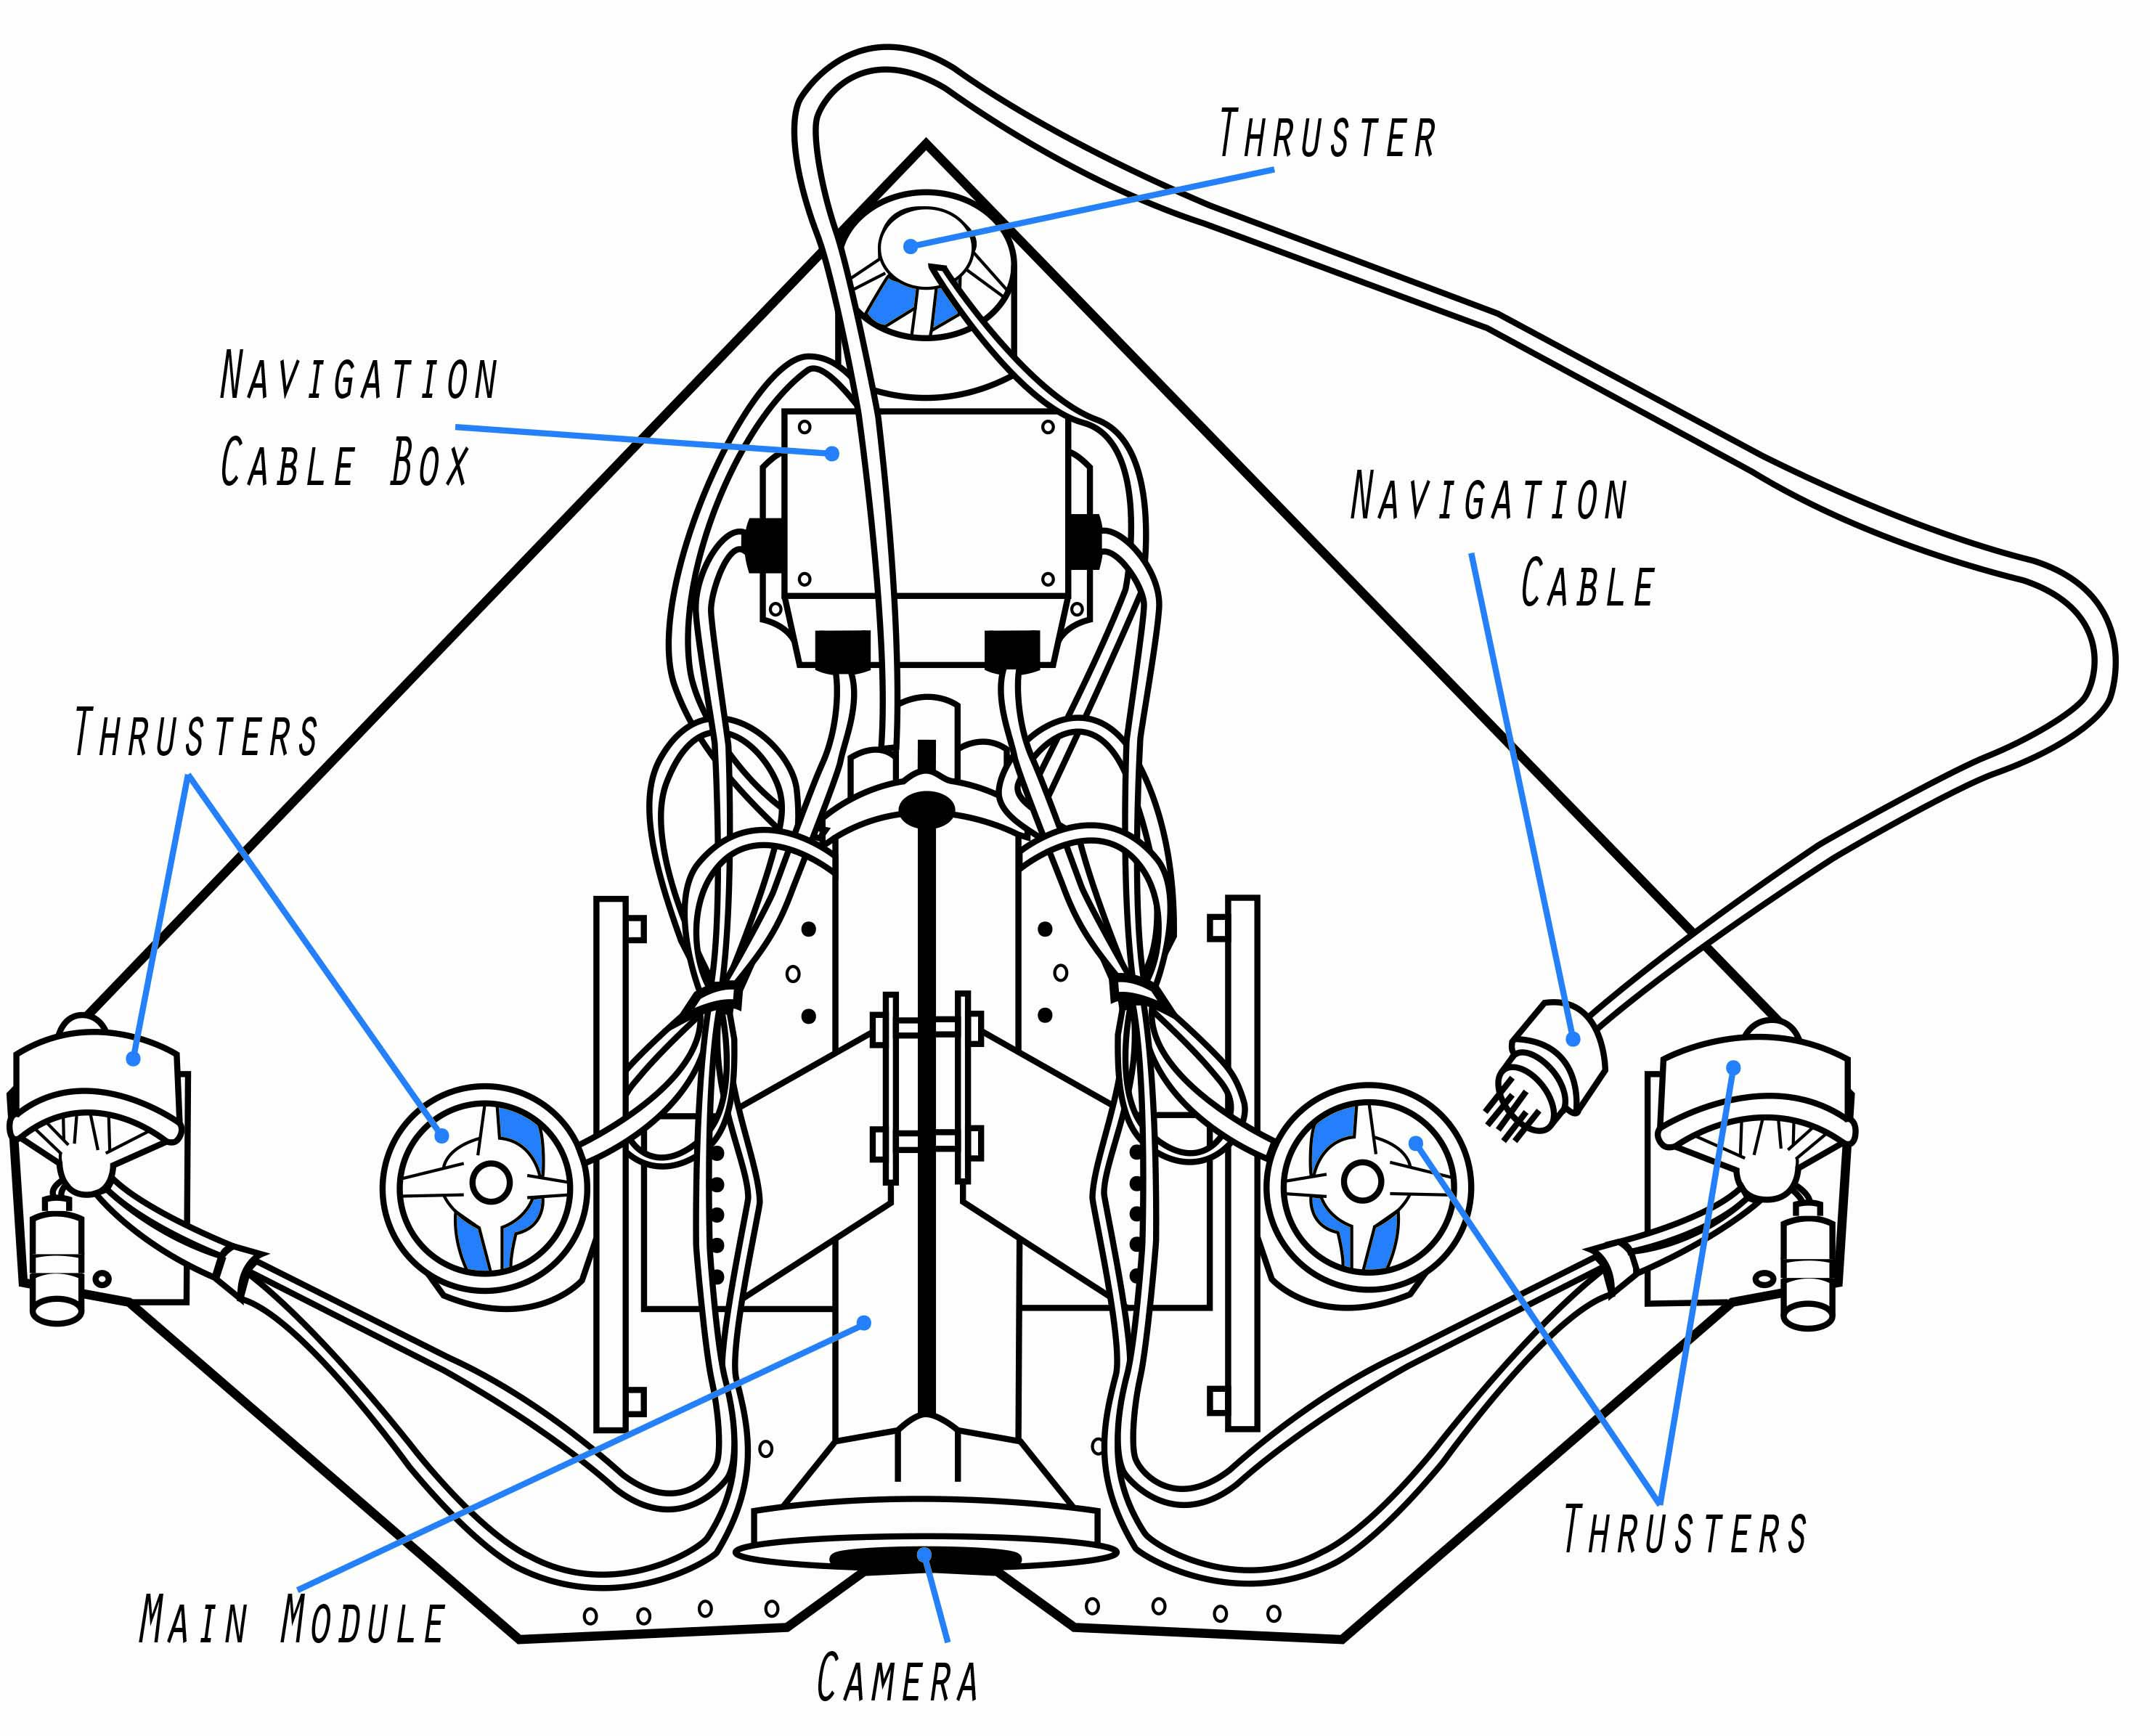
\includegraphics[width = 120mm]{assets/inside_sub.jpg}
			\caption{Proof of Design - G2X Vehicle Image 2 \label{overflow}}
		\end{figure}
	
		\begin{figure}[!htb]
			\centering
			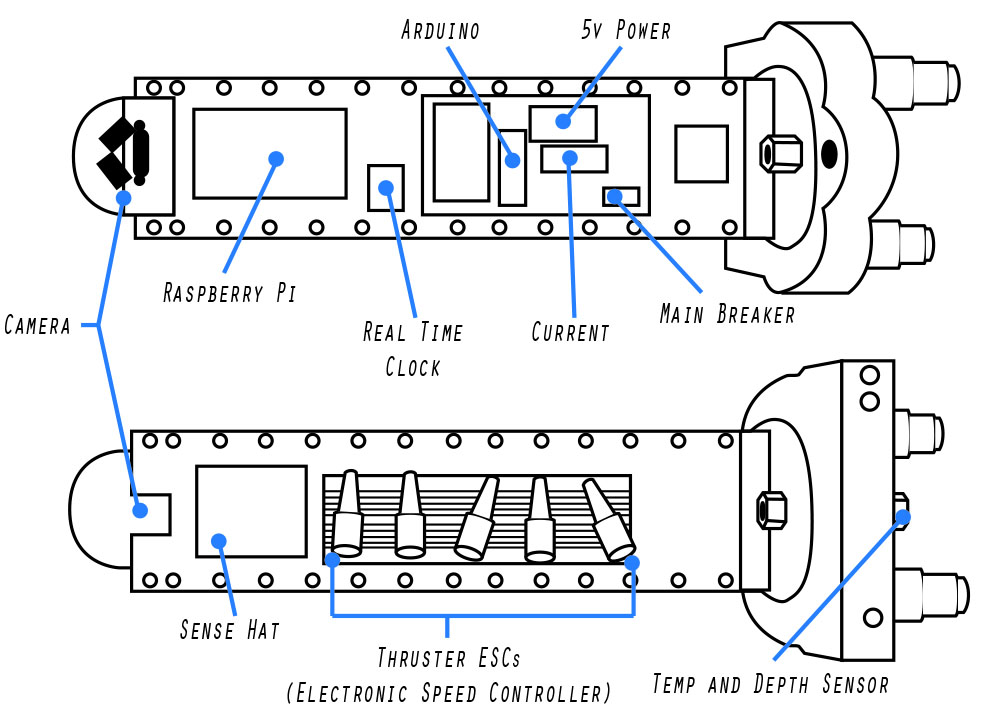
\includegraphics[width = 115mm]{assets/navigation_board.jpg}
			\caption{Proof of Design - Navigation Module \label{overflow}}
		\end{figure}
	
		\begin{figure}[!htb]
			\centering
			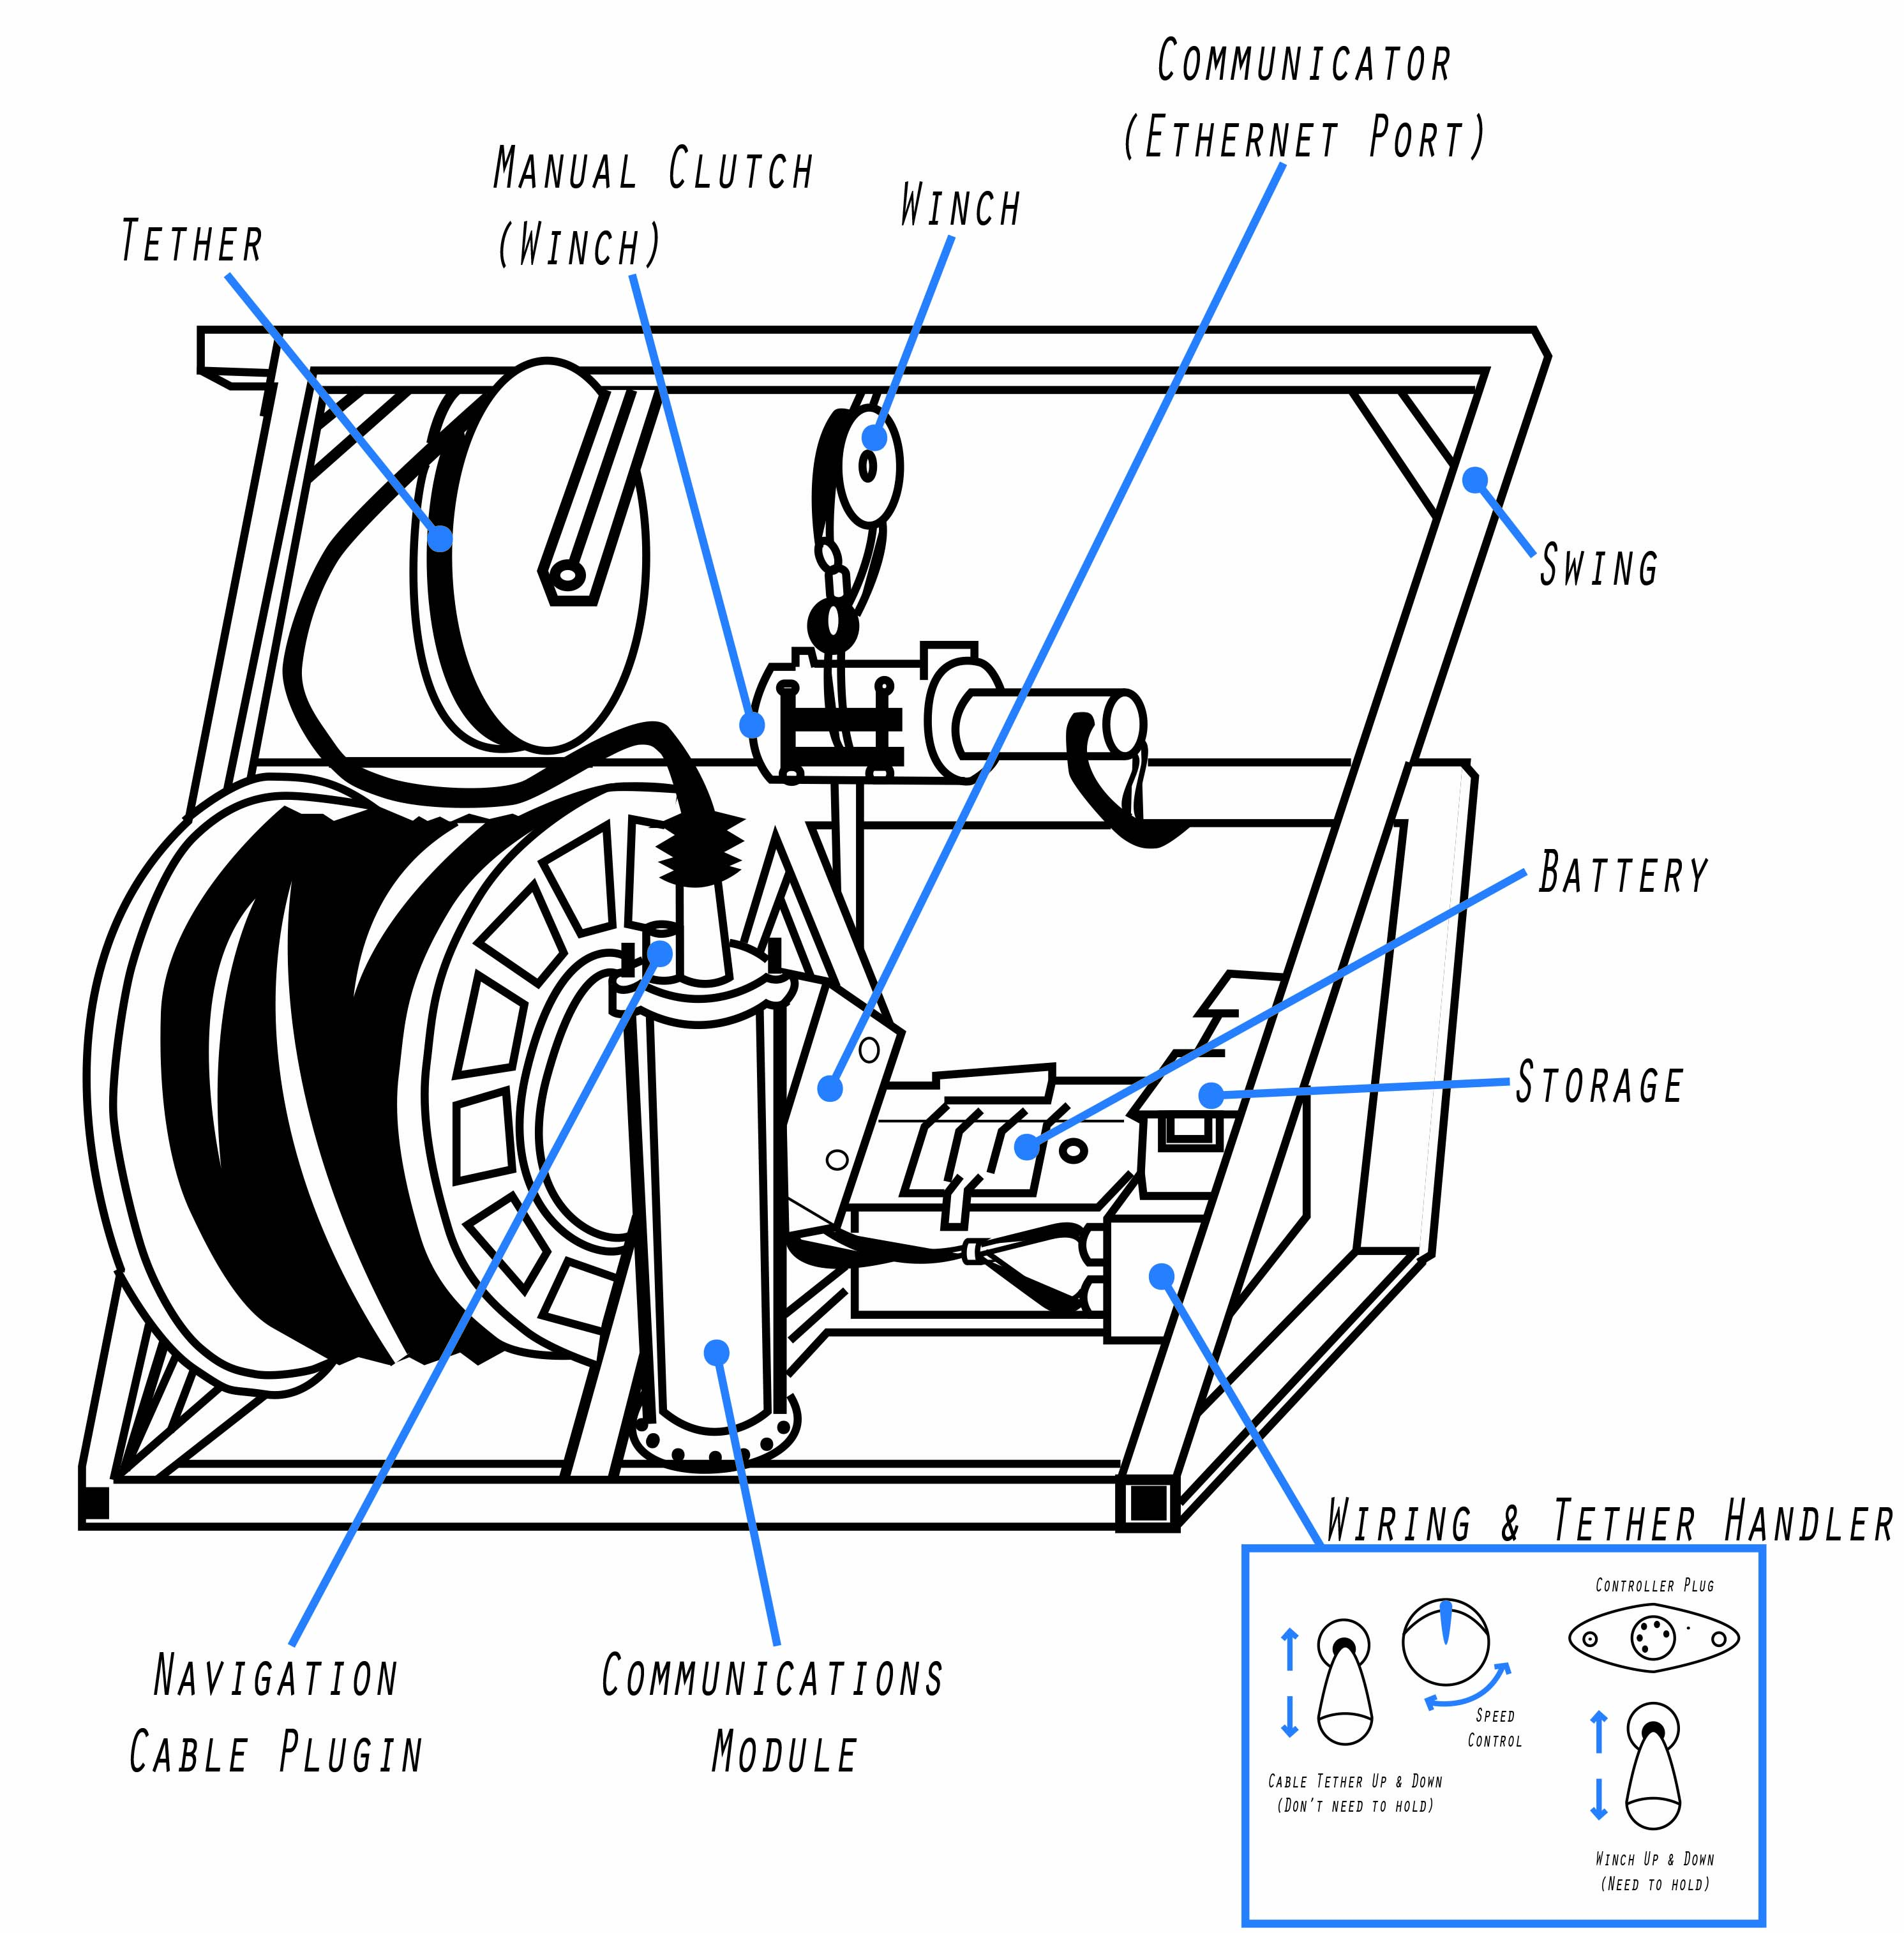
\includegraphics[width = 115mm]{assets/handling_gear.jpg}
			\caption{Proof of Design - Handling Gear \label{overflow}}
		\end{figure}
		
		% Create new Page (NEED TO USE clearpage because we have pictures that will affect it!)
		\clearpage

	\newpage
		
	\section{Design Goals}
	Client needs and project goals are discussed below. A Timeline for these is also included. Discussion of revision of goals, and addition of any new goals is also discussed below.
	
		\subsection{Original Client Needs}
		The needs of the Client (University of Idaho) are as follows:
		
		\begin{itemize}
			\item Develop and research underwater autonomous navigation software
			\item Show autonomous capability
			\item Develop wireless protocol to transmit data from sensor pod to submarine
			\item Operations manual of entire tool-chain
			\item Have tool-chain properly tested and modified for any needed fixes/changes correlating to the project
			\item Have software cooperate and be integrated with ROS
			\item Test sonar \& ROS software on TurtleBot3 as prototype
			\item Cooperate with 
			\item Documentation - both professional (team based) and personal (logbook)
			\item Complete documentation and understanding of tool-chain
			\item Configured and optimized tool-chain
			\item MQTT Wireless Protocol
			\item Catfish Logo Design
			\item Illustrations and diagrams for the entire tool-chain/system of the submarine
			\item Current \& Voltage sensor for both the Raspberry Pi and the PWM Motors
			\item Perform successful launches of the G2X submarine, both on a dock and on a boat
			\item Prototype sonar sensors (TurtleBot3)
			\item 3D print/design sonar holders on both the TurtleBot3 and the G2X Vehicle
			\item Create GitHub repository that contains all documentation, code, and additional items for the research project
			\item Laptop specifications for G2X software and additional software to run properly
			\item Work with Department of Civil and Environmental Engineering Center for Ecohydraulics Research, who which will create the sensor pod for the G2X submarine
			\item Create system diagram of all components of the project
			\item Explore tether-less options for commanding the Submarine (acoustic modem, only internal software, pinging device, etc)
			\item Linux support (ROS)
		\end{itemize}
	
			\subsubsection{Additional Client Needs}
			The additional needs of the Client (University of Idaho) that were added on as the project progressed are as follows:
			
			\begin{itemize}
				\item Modify/fix existing G2X software issues
				\item Update/edit G2X software that deals with supported controllers for the the G2X submarine
				\item Update/edit G2X software that deals with fixing the PWM Thruster overload issue (thruster lose response to Pi)
				\item Update/edit G2X software that deals with correct controller mapping for the DualShock 4 Controller on Linux Kernel 4.10+
				\item Create access point to allow for MQTT communication between Pi(Sub) and Arduino(Sensor Pod)
				\item Setup network configuration for Navigation Module Pi, Communications Module Pi on personal TP\_LINK access point, as well as static Ethernet ip on Windows/Linux computers.
				\item Add extra fuses and determine fix for blowing a fuse in the Navigation Module due to the Fiber Optic Plug
				\item Determine fix/problem for Communication Module leaking and which components suffered damage from leak
				\item Perform extra boat tests for July 26th Media Launch
				\item Determine how to properly haul gear to University of Idaho boat at Harbor Center
				\item Determine how to properly launch the submarine and retrieve the submarine from a dock/boat
				\item Check G2X software for any issues/conflicts that Websockets may present
			\end{itemize}
	
		\clearpage
	
		\subsection{Project Goal}
		The goal of this project is to develop the Coeur d'Alene Catfish, which is an autonomous robotic drone that is capable of reading water quality information from Coeur d'Alene lake, and other deep water lakes. The end result then should be the development (key word is development, not completion) of a submarine that can provide autonomous deployment within Coeur d'Alene lake and other deep water lakes. Reservoirs are also desired as well, which can be fairly difficult to navigate due to the problematic kinetic nature of the environment. This in turn allows public to the supervision of water bodies in local communities as well. The results from such surveys conducted by the drone will be shared with other interested stakeholders, this will include the Idaho Water Department of Environmental Quality (IDEQ) and Coeur d'Alene Tribe.\\
		The research focuses on creating and/or starting beginning development into the infrastructure of an autonomous submarine (and sensor technologies). Thus the long term goal is a fully functional autonomous submarine that can collect water quality data in deep-water lakes and reservoirs. The short term goal is to develop the "CDA Catfish", submarine that can perform underwater surveys by continuously sampling a variety of water quality variables (oxygen, pH, temperature, etc).\\
		Interested parties/sponsors for pursuing this research include the Idaho Water Resource Research Institute, the United States Geologic Survey, and the University of Idaho. The research is also in cooperation with Gizmo, Coeur d'Alene Maker Space.\\
		
		The product will give the user the ability to run launch the G2X submarine into a body of water and have the submarine navigate autonomously, via internal ROS software that establishes a 3D map and is either given coordinates within that map, or generates coordinates on its own to survey around the map and with these coordinates, determines a variety of routes to arrive at the location using SLAM (Simultaneous Localization and Mapping). Sonar sensors act as the eyes for the submarine, to build the map. The submarine will be expected to be tethered to received coordinate commands until a suitable/affordable tetherless alternative is discovered. G2X Software will be running on a Raspberry Pi 3B+ running Raspbian Stretch, while a remote computer will be running Ubuntu 16.04.
		
		\clearpage
		
		\subsection{Timeline}
			This is the most recent timeline for the Catfish Project:\\\\
			{ \setstretch{2.0}		
				\scalebox{1}{  		
					\begin{tabular}{r |@{\tline} l}  			
						May & Planning/Scoping/Adjustments/Finalize Program Flow         \\			
						June-July & Hardware \& Software Decision/Hardware \& Software Tinkering\\			
						August-September & Hardware/Software Implementation and Initial Prototyping\\			
						October-December & Prototype Product/Unit Testing\\			
						January-March & Product Improvement, Evaluation, and Final Product Hardware Decisions \\			
						April-June & Implementing and Producing Final Software/Hardware\\			
						July-August  & Software/Hardware Scale Testing, Software Improvements\\			
						September  & Testing\\			
						October & Ship/Delivery (Deliver product)\\			
					\end{tabular}  		
				}  	
			}
	
			\noindent \\The Gantt Chart representing our intended and actual shedule is shown in the figure below
			\begin{figure}[ht!]
				\centering
				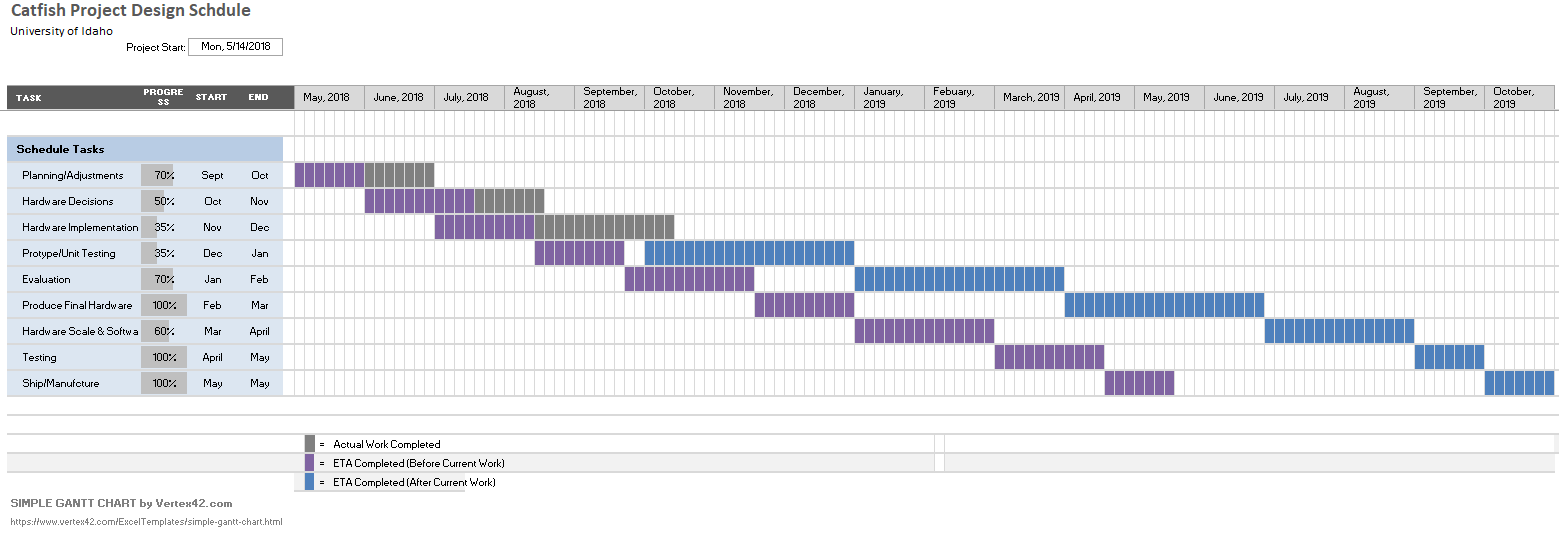
\includegraphics[width=170mm, height=85mm]{assets/Gantt_Chart.png}
				\caption{Gantt Chart - Catfish Project \label{overflow}}
			\end{figure}
		
			\clearpage	
	
	\section{Specifications and Constraints}
	Discussion of client interviews, pictures, measurements, etc. are provided below. Design specifications and constraints are also presented. Reasoning for any constraints is also mentioned.
	
	\newpage
						
	\section{System Diagrams}
	Discussion of symbols used, the diagrams themselves, and the software used for the diagrams is discussed below.
	
	\newpage				
					
	\section{Analysis of Alternatives}
	Discussion of possible alternatives and why some alternatives are better is described below. These topics include: safety, moving parts, cost, durability, compatibility, and reliability.
	
	\newpage
	
	\section{Engineering Model}
	Discussion of the physical, chemical, and biological system modeling. Also discusses modeling criteria, expected accuracy, and pitfalls. Section of modeling software used is present, as well as data needed and how the data was obtained. Lastly a validation scheme for the model is shown.
	
	\newpage
	
	\section{Manufacturing/Assembly Plan}
	Discussion of the fabrication need, a flowchart of process oriented projects, a bill of materials, and the estimated manufacturer and delivery time is discussed below.
	
	\newpage
	
	\section{Experimental Design}
	The characterization of the purpose of the experiment, model validation, data gaps, and performance measurement are discussed below. Also the details on documentation, instrumentation, and measurements are also described.
		
	\newpage	
	
	\section{Data Analysis}
	Documentation on statistical tools used, accuracy of data, and experiments shown below. Discussion on confidence is results also discussed below.
		
	\newpage
	
	\section{Balance Sheet}
	Discussion on initial budget, estimated cost for materials, components, labor, and spending plan are all described below.
		
	\newpage				
						
	\section{Other Items}
	File management, archiving, documenting any issues, reports of accidents/incidents/near misses/precautions are described below.


\end{document}
